\documentclass{article}
\usepackage{tikz}
\begin{document}

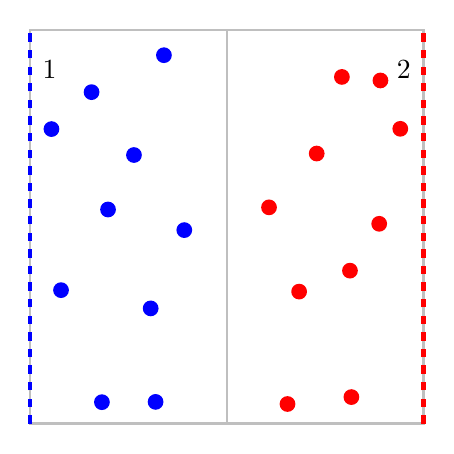
\begin{tikzpicture}

\pgfmathsetseed{18}
% Область 1 (синие точки)
\foreach \x in {0, 1} {
\foreach \y in {0,...,4}
    \fill[blue] ({\x+abs(0.75*rnd)+0.25},{\y+0.75*rnd+0.15}) circle (0.1);
}

\pgfmathsetseed{12416}
% Область 2 (красные точки)
\foreach \x in {3, 4} {
\foreach \y in {0,...,4}
    \fill[red] ({\x+rnd},{\y+rnd}) circle (0.1);
}


% Обозначения "1" и "2"
\node at (0.25,4.5) {$1$};
\node at (4.75,4.5) {$2$};



\draw[gray!50, thick] (0,0) rectangle (5,5);
\draw[thick, gray!50] (2.5, 0) -- (2.5,5);


% Границы
\draw[ultra thick, dashed, blue] (0, 0) -- (0,5);
\draw[ultra thick, dashed, red] (5, 0) -- (5,5);
\end{tikzpicture}

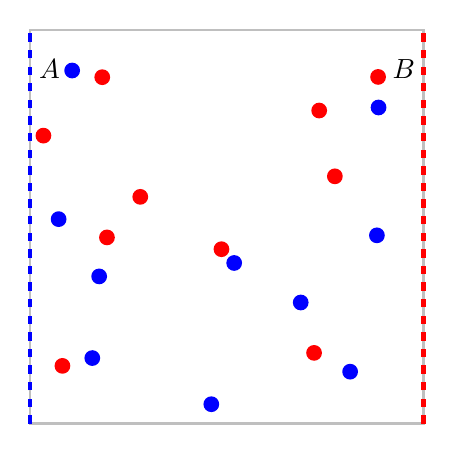
\begin{tikzpicture}

\pgfmathsetseed{685}
% Область 1 (синие точки)
\foreach \x in {1.25, 3.5} {
\foreach \y in {0,...,4}
    \fill[blue] ({\x+1.5*rand},{\y+1*rand}) circle (0.1);
}


\pgfmathsetseed{618}
% Область 2 (синие точки)
\foreach \x in {1.25,  3.5} {
\foreach \y in {0,...,4}
    \fill[red] ({\x+1.1*rand},{\y+1.5*rnd}) circle (0.1);
}


% Обозначения "1" и "2"
\node at (0.25,4.5) {$A$};
\node at (4.75,4.5) {$B$};



\draw[gray!50, thick] (0,0) rectangle (5,5);
%\draw[thick, gray!50] ({3.5/2}, 0) -- ++(0,5);


% Границы
\draw[ultra thick, dashed, blue] (0, 0) -- ++(0,5);
\draw[ultra thick, dashed, red] (5, 0) -- (5,5);

\end{tikzpicture}

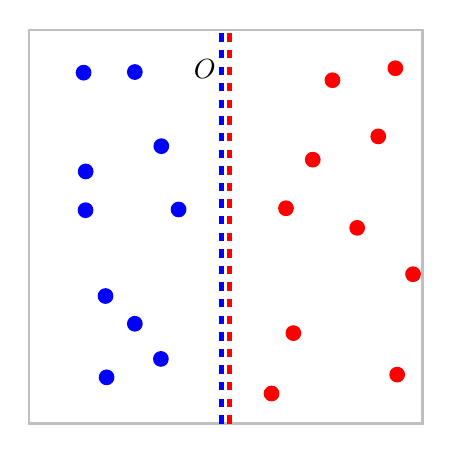
\begin{tikzpicture}

\pgfmathsetseed{20}
% Область 1 (синие точки)
\foreach \x in {0, 1} {
\foreach \y in {0,...,4}
    \fill[blue] ({\x+abs(0.75*rnd)+0.25},{\y+0.75*rnd+0.15}) circle (0.1);
}

\pgfmathsetseed{22}
% Область 2 (красные точки)
\foreach \x in {3, 4} {
\foreach \y in {0,...,4}
    \fill[red] ({\x+rnd},{\y+rnd}) circle (0.1);
}


% Обозначения "1" и "2"
\node[left] at (2.5,4.5) {$O$};
%\node at (2.75,4.5) {\LARGE 2};



\draw[gray!50, thick] (0,0) rectangle (5,5);
%\draw[thick, gray!50] (2.5, 0) -- (2.5,5);


% Границы
\draw[ultra thick, dashed, blue] (2.45, 0) -- ++(0,5);
\draw[ultra thick, dashed, red] (2.55, 0) -- ++(0,5);
\end{tikzpicture}


\end{document}
